\documentclass[../main.tex]{subfiles}

\title{Capitolo 6 - Mirror Symmetry for Landau-Ginzburg models}
\author{Edoardo Manini}
\date{Febbraio 20, 2025}

\begin{document}
\ifSubfilesClassLoaded{
\maketitle
\tableofcontents
}{}


We want to extend Mirror symmetry beyond the Calabi-Yau case. 
A Landau-Ginzburg model is a quasi-projective variety $U$ with a regular function $w \colon U \to \C$.
Following \cite{GKR17}, we are going to give a general mirror duality construction where both sides are a Landau-Ginzburg model
\[
(X,w) \longleftrightarrow  (\check{X} , \check{w}) .
\]
The varieties which will appear in the construction will be in general not necessarily smooth and not necessarily compact. In particular, they won't have a canonical Hodge structure on their cohomology groups. This is why we are going to need mixed Hodge theory if we aim to obtain a duality of Hodge numbers like the one of Batyrev for Calabi-Yau varieties.


The construction will start from a polytope $\Delta$ that is not necessarily reflexive, we will take $\check{S}$ to be the zero locus of a section of $\calO_{X_\Delta}(1)$, hence smooth. Associated to $\Delta$ we will then define two cones $\sigma$ and $\check{\sigma}$, where the former is a Gorenstein cone. We will choose desingularizations by choosing fans $\Sigma$ and $\check{\Sigma}$ which are refinements of $\sigma$ and $\check{\sigma}$ consisting only of standard cones.
We suppose that there is at least one lattice point in the interior of $\Delta$ which we will see to be equivalent to $k(\check{S})\geq 0$.
We will construct Landau-Ginzburg models, i.e. non-constant regular functions
\begin{align*}
\check{w} \colon X_{\check{\Sigma}} \to \CC \\ 
w \colon X_\Sigma \to \CC
\end{align*}
and we set $\check{S}$ to be the critical locus of $\check{w}$ which coincides with the zero locus of a section of $\calO_{X_\Delta}(1)$.
Setting $S=\mathrm{Sing} w^{-1}(0)$ and $\calF_S=\phi_w \CC[1]$ the sheaf of vanishing cycles (shifted by one), we define
\[
h^{p,q}(S, \calF_S) \defeq \dim \Gr^p_F \HH^{p+q}(S, \calF_S) = \sum_k h^{p,q+k} \HH^{p+q}(S,\calF_S)
\] 
i.e. we consider only the Hodge filtration which amounts to summing along all graded pieces of the weight filtration.
We let $d = \dim S = \dim \check{S}$, the main theorem in \cite{GKR17} is then
\begin{theorem} \textup{\cite[Thm. 5.11]{GKR17}} \label{SScheck}
    \[
    h^{p,q}(\check{S}) = h^{d-p,q}(S, \calF_S).
\]
\end{theorem}


If $g \colon X \to B$ is a proper map to a complex manifold $B$ of dim. $1$ and $b \in B$, we denote by $\psi_{g,b}$ and $\phi_{g,b}$ the functors of nearby and vanishing cycles (cfr. \ref{defNearbyVanishing}) from the category of complexes of sheaves on $g^{-1}(\DD)$ for a disk $\DD$ centered at $b$, small enough so that $b$ is the only critical value of $g$ in $\DD$. Of course, the image of the functor is independent of the size of the disk.
For $\calF^\bullet \in D^+(g^{-1}(\DD),\ZZ)$, we call $\psi_{g,b} \calF^\bullet$ (resp. $\phi_{g,b} \calF^\bullet$) the \emph{sheaf of nearby (resp. vanishing) cycles at the fibre} $b$.


We give the following definition for Hodge numbers for Landau-Ginzburg models:
\begin{defn}
     Given a complex manifold $X$ with non-constant quasi-projective regular function $w \colon X \to \C$ that has a compact critical locus, we define the Hodge numbers
     \[
h^{p,q}(X, w) = \sum_{\lambda \in \C} \dim \Gr^p_F \HH^{p+q-1}(w^{-1}(\lambda), \phi_{w,\lambda} \CC)
     \]

where $\phi_{w,\lambda}\CC$ is the sheaf of vanishing cycles at the fibre $\lambda$ and $\Gr^p_F$ is the $p$-th graded piece of its mixed Hodge structure.
\end{defn}

We have by definition:
\begin{align*}    
h^{p,q}(S, \calF_S) &= h^{p+1,q+1}(X, w), \\
h^{p,q}(\check{S}, \calF_{\check{S}}) &= h^{p+1,q+1} ( \check{X} ,\check{w}),
\end{align*}
where $X = w^{-1}(\DD)$, $\check{X} = \check{w}^{-1}(\DD)$ for $\DD$ a small disk centered at $0$ s.t. $0$ is the only critical value of $w,\check{w}$.

This follows since for $w$ 
\begin{align*}
 h^{p+1,q+1}(X ,{w}) &= \dim \Gr^{p+1}_F \HH^{p+q+1}(w^{-1}(0), \phi_{w,0} \CC) \\
 &= \dim \Gr^{p+1}_F \HH^{p+q}(w^{-1}(0), \phi_{w,0} \CC[1]) = \dim \Gr^p_F \HH^{p+q}(S, \calF_S)
\end{align*}
and similarly for $\check{w}$. In the last equality we used the fact that the filtrations on $\calF_S$ are shifted by
\begin{align*}
    F^i \calF^k_S = F^{i+1} \phi_{w,0} \CC[1], \quad \quad W_i \calF^k_S = W_{i+1} \phi_{w,0} \CC[1].
\end{align*}

Furthermore, since $\check{S}$ is smooth, the sheaf of vanishing cycles is actually just the constant sheaf $\calF_{\check{S}}[1] = \CC_{\check{S}}$ and thus $h^{p,q}(\check{S},\calF_{\check{S}}) = h^{p,q}(\check{S})$.

Hence, as a corollary of Thm. \ref{SScheck}, we have a mirror theorem for our Landau-Ginzburg models
\begin{theorem}  \textup{\cite[Cor. 5.12]{GKR17}} \label{MirrorThmLG}
    \[
    h^{p,q} (X_\Sigma,w)= h^{n-p,q}(X_{\check{\Sigma}}, \check{w}) 
    \]
    where $n = \dim X_\Sigma = \dim X_{\check{\Sigma}}$.
\end{theorem}


\subsection{The mirror construction}

We now describe the set up. Let $d$ be an integer greater than or equal to $1$. Let's fix the following notation:
\[
M \cong \ZZ^{d+1}, \quad N= \Hom(M,\ZZ) \cong \ZZ^{d+1}, \quad \overline{M} = M \oplus \ZZ, \quad \overline{N} = N \oplus \ZZ.
\]
Let $\Delta \subset M_\RR$ be a smooth lattice polytope, i.e. defining a smooth projective toric variety $X_\Delta$. Recall that this is equivalent to assume that every cone in the normal fan $\check{\Sigma}_\Delta$ of $\Delta$ is a standard cone. The normal fan $\check{\Sigma}_\Delta$ has a strictly convex piecewise linear function 
\begin{align*}
\varphi_\Delta &\colon | \check{\Sigma}_\Delta | \subset N_\RR \to \RR \\
 \varphi_\Delta(n) &\defeq    -\inf \{\langle n,m \rangle | m \in \Delta \} .
\end{align*}
Recall that $X_\Delta$ comes with an ample line bundle which we denote $\calO_{X_\Delta}(1)$, namely the line bundle associated to the divisor $D_\Delta = \sum_\rho \varphi_\Delta(n_\rho) D_\rho$ where the sum is over all rays $\rho \in \Sigma(1)$, $D_\rho$ is the prime divisor associated to the ray $\rho$ and $n_\rho$ is the unique generator of $\rho \cap N$. 

We define $\check{S}$ to be the zero locus of a section of $\calO_{X_\Delta}(1)$, hence a smooth hypersurface (by the Bertini Theorem).
We will assume that there is at least one interior lattice point of $\Delta$. This can be shown \cite[Prop. 2.14]{GKR17} to be equivalent to require that the Kodaira dimension of $\check{S}$ is $\geq 0$.
We now let 
\begin{align*}
\sigma &= \Cone(\Delta) \defeq  \{ (rm, r) | m \in \Delta, r \geq 0 \} \subset \overline{M}_\RR \\
    \check{\sigma}  &= \{ n \in \overline{N}_\RR | \langle n,m \rangle \geq 0 \quad \forall m \in \sigma \} 
\end{align*}
be a Gorenstein cone (cfr. \cite[Ex. 8.2.14]{CLS11}) and its dual.
We have $\check{\sigma} = \{ (n,r) | r \geq \varphi_\Delta(n) \} \subset \overline{N}_\RR$.

\begin{es}[Mirror dual of a genus 2 curve] \label{genus2} \mbox{}\\
    The example here is example 2.6 of \cite{GKR17}.
    Consider the two-dimensional polytope $\Delta$ in fig. \ref{Delta} with two lattice points in its interior. Its normal fan is the fan for $\PP^1 \times \PP^1$ in fig. \ref{fanP1}, i.e. $X_\Delta = \PP^1 \times \PP^1$. The zero locus $\check{S}$ of a generic section of $\calO_{X_\Delta}(1)$ is a smooth curve. Its genus is known to coincide with the number of interior lattice points of $\Delta$ \cite[Prop. 10.5.8]{CLS11}:
    \begin{align*}
        g = \dim H^0(\check{S}, \calO_{\check{S}} (K_{\check{S}})) = |\Int(\Delta) \cap M| \eqdef l^*(\Delta) ,
    \end{align*}
    which here is $2$.



\begin{figure}[ht]
  \begin{subfigure}[b]{0.4\textwidth}
    \centering 
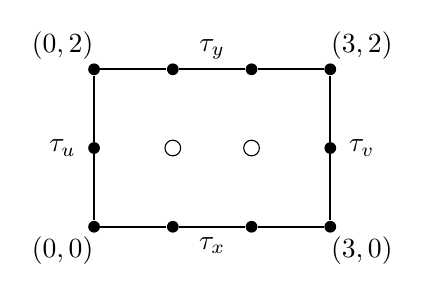
\begin{tikzpicture}[scale=1]
 \begin{scope}
        \node[circle, fill=black, inner sep=1.5pt] (D-1) at (2,1) {};
        \node[ inner sep=1.5pt] () at (2.4,1.3) {$(3,2)$};
        \node[circle, fill=black, inner sep=1.5pt] (D-2) at (1,1) {};
        \node[circle, fill=black, inner sep=1.5pt] (D-3) at (0,1) {};
        \node[circle, fill=black, inner sep=1.5pt] (D-4) at (-1,1) {};
        \node[ inner sep=1.5pt] () at (-1.4,1.3) {$(0,2)$};
        \node[circle, fill=black, inner sep=1.5pt] (D-5) at (-1,0) {};
        \node[ inner sep=1.5pt] () at (-1.4,0) {$\tau_u$};
        \node[circle, fill=black, inner sep=1.5pt] (D-6) at (-1,-1) {};
        \node[ inner sep=1.5pt] () at (-1.4,-1.3) {$(0,0)$};
        \node[circle, fill=black, inner sep=1.5pt] (D-7) at (0,-1) {};
        \node[circle, fill=black, inner sep=1.5pt] (D-8) at (1,-1) {};
        \node[circle, fill=black, inner sep=1.5pt] (D-9) at (2,-1) {};
        \node[ inner sep=1.5pt] () at (2.4,-1.3) {$(3,0)$};
        \node[circle, fill=black, inner sep=1.5pt] (D-10) at (2,0) {};
        \node[ inner sep=1.5pt] () at (2.4,0) {$\tau_v$};
        \node[circle, draw=black, inner sep=2pt] at (0,0) {};
        \node[circle, draw=black, inner sep=2pt] at (1,0) {};
        \draw[black,thick] (D-1) -- (D-2) -- (D-3) node[midway, above] {$\tau_y$} -- (D-4) -- (D-5) -- (D-6) -- (D-7) -- (D-8) node[midway, below] {$\tau_x$} -- (D-9) -- (D-10) -- (D-1);
    \end{scope}
\end{tikzpicture}
             \caption{The polytope $\Delta$}
    \label{Delta}
  \end{subfigure}
  \hfill
  \begin{subfigure}[b]{0.4\textwidth}
 \centering 
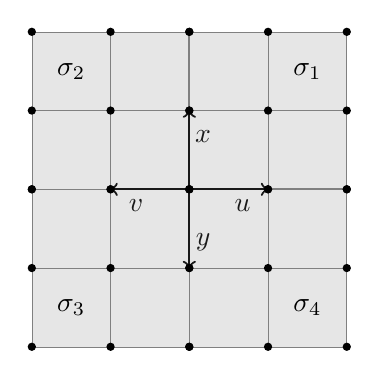
\begin{tikzpicture}
                % Draw a grid
                \draw[very thin, gray] (-2,-2) grid (2,2);
            
                % Draw the axes
                %\draw[thick,->] (-2,0) -- (2,0) node[right] {};
                %\draw[thick,->] (0,-2) -- (0,2) node[above] {};
            
                % Extend the cone's boundary (generators)
                \draw[thick,gray] (0,0) -- (2,0);
                \draw[thick,gray] (0,0) -- (0,2);
                %Generators
                \draw[thick, black, ->] (0,0) -- (1,0) node[midway, below, xshift=5pt] {$u$};
                \draw[thick, black, ->] (0,0) -- (0,1) node[midway, yshift=5pt, xshift=5pt] {$x$};
                \draw[thick, black, ->] (0,0) -- (-1,0) node[midway, below, xshift=-5pt] {$v$};
                \draw[thick, black, ->] (0,0) -- (0,-1) node[midway, yshift=-5pt, xshift=5pt] {$y$};
                
                %Fill the cones
                %sigma1
                \fill[gray,opacity=0.2] (0,0) -- (2,0) -- (2,2) -- (0,2) -- cycle;
                \foreach \x in {0,1,2} {
                    \foreach \y in {0,1,2} {
                            \fill[black] (\x,\y) circle(1.5pt);
                        }
                }
                \node at (1.5,1.5) {$\sigma_1$};
%sigma2
                \fill[gray,opacity=0.2] (0,0) -- (-2,0) -- (-2,2) -- (0,2) -- cycle;
                \foreach \x in {0,-1,-2} {
                    \foreach \y in {0,1,2} {
                            \fill[black] (\x,\y) circle(1.5pt);
                        }
                }
                \node at (-1.5,1.5) {$\sigma_2$};
%sigma3
                \fill[gray,opacity=0.2] (0,0) -- (-2,0) -- (-2,-2) -- (0,-2) -- cycle;
                \foreach \x in {0,-1,-2} {
                    \foreach \y in {0,-1,-2} {
                            \fill[black] (\x,\y) circle(1.5pt);
                        }
                }
                \node at (-1.5,-1.5) {$\sigma_3$};
%sigma4
                \fill[gray,opacity=0.2] (0,0) -- (2,0) -- (2,-2) -- (0,-2) -- cycle;
                \foreach \x in {0,1,2} {
                    \foreach \y in {0,-1,-2} {
                            \fill[black] (\x,\y) circle(1.5pt);
                        }
                }
                \node at (1.5,-1.5) {$\sigma_4$};
            \end{tikzpicture}

 \caption{Its normal fan $\check{\Sigma}_\Delta$}
    \label{fanP1}
  \end{subfigure}
  %\caption{ }
\end{figure}


    
    The piecewise linear function associated to the polytope is
    \begin{align*}
\varphi_\Delta &\colon | \check{\Sigma}_\Delta | = \RR^2 \to \RR \\
 \varphi_\Delta(n_1,n_2) &=    \left\{\begin{array}{ll} 
 0 &\quad n \in \sigma_1 \\ 
-3n_1 &\quad n \in \sigma_2 \\ 
-3n_1-2n_2 &\quad n \in \sigma_3 \\
-2n_2 &\quad n \in \sigma_4 \\
\end{array}\right.
    \end{align*}
The cone $\sigma$ has as generators the vectors $(m,1)$ for $m$ a vertex of $\Delta$, i.e.
\[
(0,0,1), \quad (3,0,1), \quad (3,2,1), \quad (0,2,1)
\]
and its dual $\check{\sigma}$ has as generators the vectors $(n_\tau, \varphi_\Delta(n_\tau))$ where $n_\tau$ is the generator of the ray of the normal fan $\check{\Sigma}_\Delta$ corresponding to the facet $\tau $ of $\Delta$., i.e.
\[
(1,0,0), \quad (0,1,0), \quad (-1,0,3), \quad (0,-1,2)
\]

\begin{figure}[ht]
  \begin{subfigure}[b]{0.4\textwidth}
    \centering 

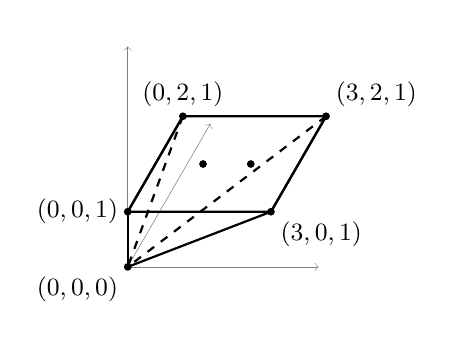
\begin{tikzpicture}[scale=0.7, isometric view/.style={x={(0.866cm,0cm)}, y={(0.5cm,0.866cm)}, z={(0cm,1cm)}}]
    \begin{scope}[isometric view]
        % Assi cartesiani
        \draw[gray, very thin, ->] (0,0,0) -- (4,0,0) node[below]{};
        \draw[gray, very thin, ->] (0,0,0) -- (0,3,0) node[right]{};
        \draw[gray, very thin, ->] (0,0,0) -- (0,0,4) node[above]{};

        % Vertici
        \coordinate (O) at (0,0,0);
        \coordinate (A) at (0,0,1); 
        \coordinate (B) at (3,0,1);  
        \coordinate (C) at (3,2,1);
        \coordinate (D) at (0,2,1);
        \coordinate (E) at (1,1,1);
        \coordinate (F) at (2,1,1);

        % Bordo inferiore
        \draw[thick] (A) -- (B) -- (C) -- (D) -- cycle;
        \draw[thick] (A) -- (O);
        \draw[thick] (B) -- (O);
        \draw[thick,dashed] (C) -- (O);
        \draw[thick,dashed] (D) -- (O);

        \draw[thick] (B) -- (A);
        \draw[thick] (C) -- (B);
        \draw[thick] (D) -- (C);
        \draw[thick] (D) -- (A);

        % Coordinate
        \node[below left] at (O) {\small$(0,0,0)$};
        \node[left] at (A) {\small$(0,0,1)$};
        \node[below right] at (B) {\small$(3,0,1)$};
        \node[above right] at (C) {\small$(3,2,1)$};
        \node[above] at (D) {\small$(0,2,1)$};

        % Punti sui vertici
        \foreach \point in {O,A,B,C,D,E,F}
            \fill (\point) circle (2pt);
    \end{scope}
\end{tikzpicture}
 \caption{The cone $\sigma=\Cone(\Delta)$}
    \label{Sigma}
  \end{subfigure}
  \hfill
  \begin{subfigure}[b]{0.4\textwidth}
 \centering 

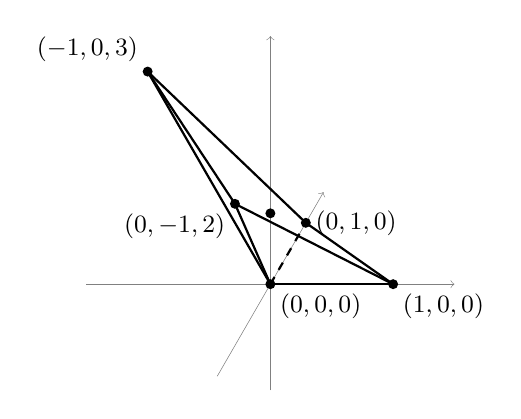
\begin{tikzpicture}[scale=0.9, isometric view/.style={x={(1.732cm,0cm)}, y={(0.5cm,0.866cm)}, z={(0cm,1cm)}}]
    \begin{scope}[isometric view]
        % Assi cartesiani (in grigio chiaro e più corti)
        \draw[gray, very thin, ->] (-1.5,0,0) -- (1.5,0,0);
        \draw[gray, very thin, ->] (0,-1.5,0) -- (0,1.5,0);
        \draw[gray, very thin, ->] (0,0,-1.5) -- (0,0,3.5);

        % Vertici
        \coordinate (O) at (0,0,0);
        \coordinate (A) at (-1,0,3);
        \coordinate (B) at (0,-1,2);
        \coordinate (E) at (0,0,1);
        \coordinate (C) at (1,0,0);
        \coordinate (D) at (0,1,0);

        % Facce del cono (ordine cruciale per la visibilità)
        
        \draw[thick,dashed] (O) -- (D);
        \draw[thick] (O) -- (C);
        \draw[thick] (O) -- (B); 
        \draw[thick] (O) -- (A);

        \draw[thick] (C) -- (D);
        \draw[thick] (B) -- (A); 
        \draw[thick] (C) -- (B);
        \draw[thick] (A) -- (D); 
      
        %Coordinate
        \node[below right] at (O) {\small$(0,0,0)$};
        \node[above left] at (A) {\small$(-1,0,3)$};
        \node[below left] at (B) {\small$(0,-1,2)$};
        %\node[above right] at (E) {\small$(0,0,1)$};
        \node[right] at (D) {\small$(0,1,0)$};
        \node[below right] at (C) {\small$(1,0,0)$};
      
        % Punti sui vertici
        \foreach \point in {O,A,B,C,D,E}
            \fill (\point) circle (2pt);
    \end{scope}
\end{tikzpicture}

 \caption{Its dual cone $\check{\sigma}$}
    \label{checksigma}
  \end{subfigure}
  %\caption{ }
\end{figure}


From this, we see that the associated toric variety $X_\sigma= \Spec (\CC[ \check{\sigma} \cap M ] )$ is
\[
X_\sigma = \Spec \left( \frac{\CC[x,y,z,u,v]}{ (xy-z^2,uv-z^3 ) } \right)
\]
where we set $z = \chi^{(0,0,1)}, x = \chi^{(0,1,0)}, y = \chi^{(0,-1,2)}, u=\chi^{(1,0,0)}, v=\chi^{(-1,0,3)}$. 
We will come back to this example later.
\end{es}

We now define refinements of the cones which will give us resolutions of singularities.
Let $\rho= (\underline{0},1) \in \overline{N}_\RR$, we see that $\rho \in \Int (\check{\sigma})$. For $\check{\sigma}$, we let
\begin{align*}
    \check{\Sigma} \defeq \Star_{\RR_{\geq0} \cdot \rho} (\check{\sigma})
\end{align*}
be the fan obtained as the star subdivision of the cone $\check{\sigma}$ along the ray $\RR_{\geq0} \cdot \rho$.
This gives a a smooth toric variety $X_{\check{\Sigma}}$.
The restriction of the projection $\overline{N} \to N$ is a map of fans $\check{\Sigma} \to \check{\Sigma}_\Delta$, hence it induces a toric morphism $X_{\check{\Sigma}} \to X_\Delta$ which is an $\AA^1$-bundle since $\check{\Sigma}$ is split by $\check{\Sigma}_\Delta$ and the ray $\RR_{\geq0} \cdot \rho$ (\cite[def. 3.3.18]{CLS11}).

Now we turn to $\sigma$. We want a refinement which gives a \emph{crepant resolution}. Such refinements arise from polyhedral decomposition $\mathscr{P}$ of $\Delta$ into lattice polytopes.
We let 
\begin{align*}
    h_* \colon \Delta \cap M &\to \ZZ \\
    h_*(m) &\defeq    \left\{\begin{array}{ll} 
 0 &\quad m \in \partial\Delta \\ 
-1 &\quad m \in \Int \Delta \\ 
\end{array}\right.
\end{align*}
and $\Delta_* = \Conv \left\{ (m,h_*(m)) | m \in \Delta \cap M \right\} \subset \overline{M}_\RR $.
Via projection to $M_\RR$ we get a subdivision of $\Delta$.

Let $\mathscr{P}_*$ be the set of faces of this subdivision. Any regular refinement of $\mathscr{P}_*$ will be called a \emph{star-like} decomposition of $\Delta$.

From now on we will assume that there is a star-like decomposition of $\Delta$ into standard simplices.
This assumption is equivalent to the assumption of the existence of a crepant resolution of the blow up at the origin of $X_\sigma$.
In general these do not necessarily exists, however they always exist if $\dim \Delta = 2$.

Note that in general there is more than one choice for $\mathscr{P}$ but as we will see, the Hodge numbers do not depend on this.

We now define the refinement $\Sigma$ of $\sigma$ by
\begin{align*}
    \Sigma \defeq \left\{ \Cone(\tau) | \tau \in \mathscr{P} \right\} \cup \{ \{0 \} \} \subset \overline{M}_\RR
\end{align*}
and similarly $\Sigma_*$ using $\mathscr{P}_*$.
We have the composition 
\begin{align*}
    X_\Sigma \to X_{\Sigma_*} \to X_\sigma
\end{align*}
where the first map is a crepant resolution and the second one is a blow up.

\begin{es}
    If $\Delta$ is a reflexive polytope, we have $\check{\sigma} = \Cone(\Delta)^\vee = \Cone(\Delta^\circ)$ and in this case $\mathscr{P}_*$ is the Star subdivision of $\Delta$ at $0$.
\end{es}

We can now choose Landau-Ginzburg potentials:
\begin{align*}
    w \colon X_{\Sigma} &\to \CC \\
    \check{w} \colon X_{\check{\Sigma}} &\to \CC 
\end{align*}
First observe that 
\begin{align*}
    \check{\Sigma}(1) = \left\{ \rho =(\underline{0},1), (n_\tau,\varphi_\Delta(n_\tau)) \right\}_{\tau \in \text{Facets}(\Delta)}
\end{align*}
where $n_\tau$ is the generator of the ray of the normal fan $\check{\Sigma}_\Delta$ corresponding to the facet $\tau $ of $\Delta$.
Hence we take
\begin{align*}
    w = c_\rho \chi^\rho + \sum_{\substack{\tau \subset \Delta \\ \codim (\tau)=1 } } c_\tau \chi^{\left( n_\tau,\varphi_\Delta(n_\tau) \right)}
\end{align*}
Second, since $\Sigma(1)= \left\{ (m,1) \right\}_{m \in \Delta \cap M}$, we write:
\begin{align*}
    \check{w} = \sum_{m \in \Delta \cap M} c_m \chi^{(m,1)}
\end{align*}

Define $\check{S} = \crit(\check{w})$.

\begin{rem}
Giving $\check{w}$ is equivalent to give a section 
\[
\check{s} \in H^0 \left( X_\Delta,\calO_{X_\Delta} (1) \right) = \bigoplus_{m \in \Delta \cap M} \CC \cdot \chi^m:
\]
\begin{align*}
    \check{w} = \sum_{m \in \Delta \cap M} c_m \chi^{(m,1)} \quad  \stackrel{\sim}{\longleftrightarrow} \quad \check{s} = \sum_{m \in \Delta\cap M} c_m \chi^m
\end{align*}
and $\check{S}=\crit(\check{w})$ coincides with the zero locus of $\check{s}$. Indeed $p \in \crit(\check{w})$ iff $d\check{w}(p)=\underline{0}$. If we let $z = \chi^\rho = \chi^{(\underline{0},1)}$, we have $\check{w}=z \cdot \check{s}$ and
\begin{align*}
    d\check{w} = \left( \frac{\partial\check{w}}{\partial \chi^m}, \frac{\partial \check{w}}{\partial z} \right) = \left( z \frac{\partial\check{s}}{\partial \chi^m}, \check{s} \right) , 
\end{align*}
hence $\check{S}=\crit(\check{w}) = \{ z=0,  \check{s} =0 \}$.
\end{rem}

The maps $w, \check{w}$ are not proper, still one can find properifications by choosing fans $\overline{\check{\Sigma}}$ and $\overline{{\Sigma}}$ that are complete and give projective compactifications in such a way that the maps 
\[
  w \colon X_{\Sigma} \to \CC \qquad \check{w} \colon X_{\check{\Sigma}} \to \CC 
\]
become quasi-projective (see \cite[Cor. 2.10]{GKR17}). In fact $w$ and $\check{w}$ extend to give projective morphisms
\begin{align*}
\bar{w} \colon \Tilde{\bar {X}} \to \PP^1    \qquad \bar{\check{w}} \colon \Tilde{\bar{\check{X}}} \to \PP^1
\end{align*}
where $\Tilde{\bar {X}}$ and $\Tilde{\bar{\check{X}}}$ are smooth compact projective toric varieties containing $ X_{\Sigma}$ and $X_{\check{\Sigma}}$ as open subsets (see \cite[Prop. 2.8, 2.9]{GKR17}).


We set
\begin{align}
     W_t \defeq \overline{w^{-1}(t) \cap (\CC^*)^{d+2}}
\end{align}
where the overline denotes the closure in $X_\Sigma$.
By \cite[Prop. 2.20]{GKR17}, we have $w^{-1}(t) = W_t$ for $t \neq 0$ and
\begin{align*}
w^{-1}(0) = W_0 \cup \bigcup_{v \in \Int(\Delta) \cap M} D_v
\end{align*}
is normal crossings. $W_0$ is the component of $w^{-1}(0)$ which is not contained in any toric stratum of $X_\Sigma$.
Hence $w^{-1}(0)$ is a union of divisors and $S = \Sing w^{-1}(0)$ is the intersection of such divisors. In the case of Ex. \ref{genus2}, $w^{-1}(0)$ is a normal crossing union of three surfaces $W_0, D_1, D_2$ and $S = \Sing w^{-1}(0)$ is topologically a configuration of three projective lines intersecting in two triple points. See fig. \ref{g2mirror}.


\begin{figure}[h!]
\centering
    \includegraphics[width=8cm]{images/Genus_2_Mirror.png}
    \caption{Mirror of a genus 2 curve}
    \label{g2mirror}
\end{figure}


%
%
%
%Given $\tau \in \mathscr{P}$, let $\mathscr{P}_*(\tau)$ denote the %smallest cell of $\mathscr{P}_*$ containing $\tau$.

%\begin{defn}
%    A $k$-dimensional handlebody $H^k$ is the intersection $H^k = H %\cap (\CC^*)^{k+1}$ of a general hyperplane $H$ in $\PP^{k+1}$.
%\end{defn}

%We have:
%\begin{proposition}\textup{\cite[Cor. 2.21]{GKR17}}
%For $\tau \in \mathscr{P}, \tau \subset \partial \Delta$, denoting %by $T_\tau$ the torus orbit of $X_\Sigma$ corresponding to %$\Cone(\tau)$, we have
%\begin{align*}
%w^{-1}(t) \cap T_\tau &\simeq H^{\codim \mathscr{P}_*(\tau)-1} %\times (\CC^*)^{\dim \mathscr{P}_*(\tau) - \dim \tau} \quad \text{ %for } t \neq 0, \\
%w^{-1}(0) \cap T_\tau &\simeq H^{\codim \mathscr{P}_*(\tau)-2} %\times (\CC^*)^{\dim \mathscr{P}_*(\tau) - \dim τ+1} 
%\end{align*}
%where $\codim  \mathscr{P}_*(\tau) = d + 1- \dim \mathscr{P}_*%%(\tau)$. 
%\end{proposition}




%\subsection{Hodge numbers of hypersurfaces in projective toric %varieties}

%In this section we recall some results on Hodge numbers of %hypersurfaces in projective toric varieties from \cite{DK86}.

%As we have seen in section \ref{mhssmooth}, Deligne showed that for %a complex algebraic variety $X$, the cohomology $H^k(X,\QQ)$ carries %a natural mixed Hodge structure. However, for the purpose of the %following. it is more convenient to use cohomology with compact %support $H^k_c(X,\QQ)$. 
%In particular ordinary cohomology does not behave well with respect %to the relations for the Grothendieck group $K_0(\mathrm{Var})$:
%\[
%[X]= [X \setminus Y] + [Y].
%\]
%Cohomology with compact support also carry a natural mixed Hodge %structure. It is given via the isomorphism $H^k_c(U) %\xrightarrow{\sim} H^k(X,D)$, where $U \hra X $ is a good %compactification of $U$ and $D \defeq X \setminus U$. Let $j \colon %X \setminus U \hra X$, then the MHS on $H^k(X,D)$ is given by the %mixed cone $\Cone^\bullet(j^*)$.

%It is not hard to prove the following properties regarding mixed %Hodge theory for cohomology with compact support of smooth algebraic %varieties analogous to the ones for ordinary cohomology:
%\begin{enumerate}
    %\item if $f \colon X \to Y$ is proper, then $f^* \colon %H^\bullet_c(Y) \to H^\bullet_c(X)$ is a morphism of MHS
    %\item if $Y \subset X$ is closed, then
    %\[
    %\cdots \lra H^k_c(X \setminus Y) \lra H^k_c(X) \lra H^k_c(Y)% %\lra H^{k+1}_c(X \setminus Y) \lra \cdots 
%    \]
%    is a long exact sequence of MHS.
%    \item $h^{p,q}H^k_c(X) = 0$ for $p+q >k$.
%\end{enumerate}

%\begin{defn}
    %For a complex algebraic variety $X$, the $(p,q)$-th and the $p$-%th compactly supported Hodge-Deligne numbers are defined as
%    \begin{align*}
%        e^{p,q}_c(X) &\defeq \sum_k (-1)^k h^{p,q}[H^k_c(X)] \\
%        e^p_c(X) &\defeq \sum_q e^{p,q}(X)
%    \end{align*}
%\end{defn}
%The $e^{p,q}_c(X)$ are the coefficients of the compactly supported %Hodge-Euler polynomial 
%\[
%e(X) = e_{Hdg}^c(X) \defeq \sum_k (-1)^k h^{p,q}[H^k_c(X)] u^pv^q  %\in \ZZ[u,v] .
%\]
%If $X$ is smooth and compact we have that the $e^{p,q}_c(X)$ %coincide with the Hodge numbers up to sign
%\[
%e^{p,q}_c(X)=(-1)^{p+q}h^{p,q}(X)
%\]
%
%An important reason to introduce $e(X)$ is the following property %which we will need later.
%
%\begin{proposition} \textup{\cite[Prop. 1.6]{DK86}}
    %Suppose that $X = \bigsqcup_i X_i$ is a disjoint union of a %finite number of locally closed subvarieties $X_i, \quad i \in %I$. Then 
%    \[
%    e(X) = \sum_{i \in I} e(X_i).
%    \]
%\end{proposition}
%\begin{cor} \textup{\cite[Cor. 1.7]{DK86}}
    %Let $\{ X_i \}$ be a finite covering of $X$ by locally closed %subvarieties. Then
%    \[
%e(X) = \sum_{i_o< \cdots < i_k } (-1)^k e(X_{i_0} \cap \cdots \cap %X_{i_k} ).
%    \]
%\end{cor}%

%The following useful property follows immediately from the Kunneth %formula.
%\begin{proposition}
   % \[
  %  e(X \times Y) = e(X) \times e(Y)
 %   \]
%\end{proposition}
%
%\begin{es}
%If $X=\{*\}$ is a point, then $e(X)=e(\{*\}) = 1$.
%
%For $\PP^1$ we know $e(\PP^1)=1 + uv$.
%Since $\PP^1 = \CC \bigsqcup \{\infty \}$, in the Grothendieck group %$K_0(Var)$ we have $[\PP^1] = [\CC] + [\{\infty\}]$, therefore
%\[
%e(\CC) = uv
%\]
%Similarly for $\CC \setminus \{0 \}$, we have $e(\CC \setminus \{0 %\}) = uv-1$.
    %Let $\TT^n = (\CC \setminus \{0\})^n$ be the algebraic torus. %Then 
   % \[
   % e(\TT^n)=(uv-1)^n
    %\]
    %from the previous proposition and the fact that $e(\CC \setminus %\{0\})=uv-1$.
%\end{es}
%    
%In the previous section we have seen that toric varieties have the %nice property to be the disjoint unioin of torus orbits.
%In particular for a toric variety coming from a polytope $X_\Delta$, %we have a torus $\TT_F$ for every face $F \subset \Delta$ of %$\Delta$.
%Using this fact we can prove 
%\begin{cor}
    %For $X_\Delta$ a smooth toric variety coming from a polytope of %maximal dimension,
%    \begin{align*}
%        h^{p,q}(X_\Delta)=  \left\{\begin{array}{ll} 
% 0 &\quad p \neq q \\ 
%(-1)^p \sum_{F \in \mathrm{Faces}(\Delta)} (-1)^{\dim F} {\dim %F\choose{p}}  &\quad m \in \Int \Delta \\ 
%\end{array}\right.
%    \end{align*}
%\end{cor}
%\begin{proof}
%The vanishing of $h^{p,q}(X_\Delta)$ for $p \neq q$ is a consequence %of the vanishing result \cite[Thm. 9.3.2]{CLS11}.
    %Since $X_\Delta= \bigcup_{F \subset \Delta} \TT_F $ is a union %of tori, $e(X_\Delta)=\sum_{F \subset \Delta} (uv-1)^{\dim F}$. %$X_\Delta$ is smooth and compact so $h^{p,q}(X_\Delta)= %(-1)^{p+q}e^{p,q}_c(X_\Delta)$. Therefore
    %\[
    %h^{p,p}(X_\Delta)= e^{p,p}(X_\Delta)=\sum_{F \subset \Delta} %(-1)^{\dim F - p}  {\dim F\choose{p}}
%    \]
%\end{proof}

%Take $\Delta$ a smooth polytope of maximal dimension $d+1$. Assume %there is a polyhedral decomposition $\mathscr{P}$ of $\Delta$ into %standard simplices. Let $\check{s} \in H^0(X_\Delta,\calO_{X_\Delta}%(1))$ and $\check{S} = \{\check{s}=0 \}$ a smooth hypersurface in %$X_\Delta$ as before.

%The following proposition, coming from results by Danilov and %Khovanskii \cite{DK86}, tells us how to calculate the Hodge numbers %of a smooth toric hypersurface. 

%\begin{proposition} \textup{\cite[Prop. 3.2]{GKR17}}
    %\begin{enumerate}
        %\item  $h^{p,q}(\check{S}) = 0$ unless $p = q$ or $p + q = %d$.
        %\item For $\tau \in \mathscr{P}$, let $\Delta(\tau)$ be the %minimal face of $\Delta$ containing $\tau$. Then
%        \begin{align*}
%(-1)^pe^p(\check{S}) = \sum_q (-1)^q h^{p,q}(\check{S}) = &-%\sum_{\tau \subset \Delta} (-1)^{ \dim \tau} {\dim τ \choose{p + 1}} % \\
%&+ \sum_{\tau \in \mathscr{P} } (-1)^{ \dim \tau} { \dim %\Delta(\tau) - \dim \tau \choose{p + 1}}
        %\end{align*}
        %\item For $2p > d$, 
        %\[
        %h^{p,p}(\check{S}) = h^{p+1,p+1}(X_\Delta) = (-1)^{p+1} %\sum_{ \tau \subset \Delta} (-1)^{ \dim \tau} { \dim \tau %\choose{p+1}}
        %\]
        %and
        %\[
        %h^{p,d-p}(\check{S}) = \sum_{\tau \in \mathscr{P}} (-1)^{d-%p+ \dim \tau} {\dim \Delta(\tau) - \dim \tau \choose{p + 1}}
%        \]
%    \end{enumerate}
%\end{proposition} %

%To calculate the Hodge numbers of the mirror $S$ we will need the %following proposition about the Hodge-Deligne numbers of a product %of a handlebody $H^k=H \cap (\CC^*)^{k+1} \subseteq \PP^{k+1}$ and a %torus $(\CC^*)^l$.
%We have:
%\begin{proposition} \textup{\cite[Lem. 3.4]{GKR17}}
%    \begin{align*}
%        e^{p,q}(H^k \times (\CC^*)^l) =  \left\{\begin{array}{ll} 
% 0 &\quad p \neq q \\ 
%(-1)^{p+k+l} \left(  {k + l + 1 \choose{p + 1}} - {l \choose{p + 1}} % \right) &\quad p=q \\ 
%\end{array}\right. 
%    \end{align*}
%\end{proposition}

%\subsection{The Hodge numbers of the mirror}

\subsection{Mirror dual of a genus 2 curve}

In this section we explicitly calculate the Hodge numbers of the mirror dual of a genus $2$ curve as given in \cite{GKR17} using the spectral sequence for the complex of vanishing cycle and we verify the \emph{Mirror} symmetry for the Hodge diamonds.

We consider the set up of example \ref{genus2}.
We have the planar polytope $\Delta$ with $2$ interior lattice points. We have seen that the hypersurface $\check{S} $ is a smooth genus $2$ curve.

For $S$ on the other side, we know that it is a configuration of three projective lines meeting in $2$ triple points. See fig. \ref{g2mirror}.

%Choose a small disk $\DD \subset \CC \subset \PP^1$ centered at $0 %\in \CC$ which does not contain any other critical values of %$\bar{w}$ and consider the restriction
%\[
%\bar{w} \colon \bar{w}^{-1}(\DD) \to \DD
%\] 
%We set $\bar X = \bar w^{-1}(\DD), \quad X = X_\Sigma \cap \bar X, %\quad \bar w \colon \bar X \to \DD$,

We want to calculate
\begin{align} \label{hpqdefinition}
h^{p,q}(S, \calF_S) \defeq \dim \Gr^p_F \HH^{p+q}(S, \calF_S) = \sum_k h^{p,q+k} \HH^{p+q}(S,\calF_S).
\end{align}

In order to do that we first notice that 
\begin{align*}
    \HH^{m}(S, \calF_S) = \HH^{m}(Y, \phi_w \CC_X[1]) = \HH^{m+1}(Y, \phi_w \CC_X) = \HH^{m+1}(Y, \bar A^\bullet)
\end{align*}
where $Y \defeq w^{-1}(0)$ is a n.c.d. in $X=X_\Sigma$ and $\bar A^\bullet$ is the complex of sheaves quasi-isomorphic to $\phi_w \CC_X$ we defined in sect. \ref{Sect.CMHC.LMHS}. 

Also notice the shift in the definition of $\calF_S$ corresponds to shifts in the filtrations:
\begin{align*}
    F^i\calF^k_S = F^{i+1} \bar A^{k+1}, \\
    W^i \calF^k_S = W^{i+1} \bar A^{k+1}
\end{align*}
which imply
\begin{align} \label{shiftHdgnumbers}
    h^{p,q} \HH^i (S, \calF_S) = h^{p+1,q+1} \HH^{i+1}(Y, \phi_w \CC_X)
\end{align}


Recall the spectral sequence \eqref{Wspecseq} 
\begin{equation} \label{spseqAbar}
E^{-k,m+k}_1=\HH^{m}(X,\Gr^{W(M)}_{k}\bar A^\bullet) \Rightarrow \HH^{m}(X,\bar A^\bullet).
\end{equation}
whose first page, via Poincarè residue isomorphisms, can be written as
\begin{align}
E^{-k,m+k}_1=\bigoplus_{q>-1,-k} H^{m-2q-k}( Y({2q+k+1}),\CC)(-q-k).  
\end{align}
Recall also the morphisms $d_1$ in the first page, given by $\delta-\gamma$.

Here $Y(1)$ is a disjoint union of three surfaces which we denote by $Y_1,Y_2,Y_3$, while $Y(2)$ is a disjoint union of three copies of $\PP^1$ which we denote by $Y_{12},Y_{23},Y_{13}$ and $Y(3)$ are the two triple points which we denote $\{a,b\}$.

We have inclusions
\begin{align*}
    \delta_1^3 \colon \{a,b\} \hra Y_{23} \\
    \delta_2^3 \colon \{a,b\} \hra Y_{13} \\
    \delta_3^3 \colon \{a,b\} \hra Y_{12} 
\end{align*}
which we consider as maps from $Y(3)$ to $Y(2)$.


We notice that the only non-trivial groups in the first page of \eqref{spseqAbar} are
\begin{align*}
      E_1^{-k,m+k} = \left\{\begin{array}{ll} 
 H^0(Y(2),\CC)(-1) &\quad k=m=1 \quad (q=0) \\ 
H^0(Y(3),\CC)(-1) &\quad k=0, \quad m=2 \quad (q=1)  \\ 
H^0(Y(3),\CC)(-2) &\quad k= m=2 \quad (q=0) \\ 
 H^2(Y(2),\CC)(-1) &\quad k=1, \quad m=3 \quad (q=0) \\ 
\end{array}\right.
\end{align*}

The $E_1^{\bullet,\bullet}$-page of the spectral sequence is then
 
\begin{center}
\begin{tikzpicture}
  \matrix (m) [matrix of math nodes,
    nodes in empty cells,nodes={minimum width=5ex,
    minimum height=5ex,outer sep=-5pt},
    column sep=1ex,row sep=1ex]{
          4     & \C^2 & \C^3 &  0   & \\
          3     &  0   &  0   &  0   & \\
          2     &  0   & \C^3 & \C^2 & \\
    \quad\strut &   -2  &  -1  &  0  & \strut \\};
  \draw[-stealth] (m-3-3.east) -- node[anchor=south] {$\delta$} (m-3-4.west) ;  
  \draw[-stealth] (m-1-2.east) -- node[anchor=south] {$-\gamma$} (m-1-3.west) ;
\draw[thick] (m-1-1.east) -- (m-4-1.east) ;
\draw[thick] (m-4-1.north) -- (m-4-5.north) ;
\end{tikzpicture}
\end{center}

where the differential $E_1^{-1,2}=H^0(Y(2),\C) \to E_1^{0,2}=H^2(Y(3),\C)$ is the restrction map $\delta$, i.e.
\begin{align*}
    H^0(Y(2))=\langle [1_{Y_{12}}], [1_{Y_{23}}],[1_{Y_{13}}] \rangle &\xrightarrow{\delta \defeq {\delta_1^3}^*-{\delta_2^3}^* +{\delta_3^3}^*} H^0(Y(3))=\langle [1_a], [1_b] \rangle \\
    1_{Y_{12}} &\longmapsto 1_a \oplus 1_b \\
     1_{Y_{23}} &\longmapsto 1_a \oplus 1_b \\
      1_{Y_{13}} &\longmapsto -1_a \oplus -1_b 
\end{align*}
In other words the linear map represented by the matrix
$\begin{pmatrix}
1  & 1 & -1 \\
1  & 1 & -1 
\end{pmatrix}$. \\
The differential $E_1^{-2,4}=H^0(Y(3),\C) \to E_1^{-1,4}=H^2(Y(2),\C)$ is the Gysin map $-\gamma$, i.e.
\begin{align*}
    H^0(Y(3))=\langle [1_a], [1_b] \rangle &\xrightarrow{-\gamma \defeq -{\delta_1^3}_! + {\delta_2^3}_! -  {\delta_3^3}_!  } H^2(Y(2))=\langle [{Y_{12}}], [{Y_{23}}],[{Y_{13}}]\rangle \\
    1_a &\longmapsto  - [{Y_{12}}] \oplus - [{Y_{23}}] \oplus [{Y_{13}}] \\
    1_b &\longmapsto  - [{Y_{12}}] \oplus - [{Y_{23}}] \oplus [{Y_{13}}]
\end{align*}
These two maps have both kernel of dimension one,
so the $E_2^{\bullet,\bullet}$-page looks like 
\begin{center}
\begin{tikzpicture}
  \matrix (m) [matrix of math nodes,
    nodes in empty cells,nodes={minimum width=5ex,
    minimum height=5ex,outer sep=-5pt},
    column sep=1ex,row sep=1ex]{
          4     & \C & \C^2 &  0   & \\
          3     &  0   &  0   &  0   & \\
          2     &  0   & \C^2 & \C & \\
    \quad\strut &   -2  &  -1  &  0  & \strut \\};
\draw[thick] (m-1-1.east) -- (m-4-1.east) ;
\draw[thick] (m-4-1.north) -- (m-4-5.north) ;
\end{tikzpicture}
\end{center}
In other words 
\[
 {E_2^{-k,m+k}}= \Gr^{W(M)}_{m+k} \HH^m(X,\bar A^\bullet)=
    \left\{\begin{array}{ll} 
 \CC^2 &\quad k = m = 1 \\ 
 \C &\quad k = 0, \quad m = 2 \\
  \C &\quad k = m = 2 \\
  \CC^2 &\quad k =1, \quad m = 3 \\
0 &\quad \text{otherwise}  \end{array}\right.
\]
Taking the sum along the anti-diagonals, we obtain
\[
\HH^i(Y, \bar A^\bullet)= \left\{\begin{array}{ll} 
 \C^2 &\quad i = 1,2,3 \\ 
0 &\quad \text{otherwise} . \end{array}\right.
\]


We also obtain the following Hodge numbers
\begin{eqnarray*}
h^{p,q}\HH^3(\bar A^\bullet)&=  \dim \Gr^p_F \Gr^{W(M)}_{p+q} \HH^3(\bar A^\bullet)  &=
\left\{\begin{array}{ll} 2 &\quad p=q=2\\ 0&\quad\hbox{otherwise,}\end{array}\right.\\
h^{p,q}\HH^2(\bar A^\bullet)&= \dim \Gr^p_F \Gr^{W(M)}_{p+q} \HH^2(\bar A^\bullet)   &=
\left\{\begin{array}{ll} 1 &\quad p=q=1\hbox{ or }p=q=2\\ 0&\quad\hbox{otherwise,}\end{array}\right.\\
h^{p,q}\HH^1(\bar A^\bullet)&= \dim \Gr^p_F \Gr^{W(M)}_{p+q} \HH^1(\bar A^\bullet)  &=
\left\{\begin{array}{ll} 2 &\quad p=q=1\\ 0&\quad\hbox{otherwise.}\end{array}\right.
\end{eqnarray*}

where to calculate these numbers we used the fact that the Hodge $F$ filtration has to be shifted because of the presence of the Tate twist ($F^p H(r) = F^{p+r} H$).

By \eqref{shiftHdgnumbers}, we obtain
\begin{eqnarray*}
h^{p,q}\HH^2(S, \calF_S)&=  \dim \Gr^p_F \Gr^{W(M)}_{p+q} \HH^2(S, \calF_S)  &=
\left\{\begin{array}{ll} 2 &\quad p=q=1\\ 0&\quad\hbox{otherwise,}\end{array}\right.\\
h^{p,q}\HH^1(S, \calF_S)&= \dim \Gr^p_F \Gr^{W(M)}_{p+q} \HH^1(S, \calF_S)   &=
\left\{\begin{array}{ll} 1 &\quad p=q=0 \hbox{ or }p=q=1\\ 0&\quad\hbox{otherwise,}\end{array}\right.\\
h^{p,q}\HH^0(S, \calF_S)&= \dim \Gr^p_F \Gr^{W(M)}_{p+q} \HH^0(S, \calF_S)  &=
\left\{\begin{array}{ll} 2 &\quad p=q=0\\ 0&\quad\hbox{otherwise.}\end{array}\right.
\end{eqnarray*}

This in turn implies, using definition \eqref{hpqdefinition} of $h^{p,q}(S,\calF_S)$ :
\begin{align*}
    h^{0,0}(S,\calF_S)= h^{0,0}\HH^0(S, \calF_S) + h^{0,1}\HH^0(S, \calF_S) + \dots  = 2 \\
    h^{1,0}(S,\calF_S)= h^{1,0}\HH^1(S, \calF_S) + h^{1,1}\HH^1(S, \calF_S) + \dots = 1 \\
     h^{0,1}(S,\calF_S)= h^{0,0}\HH^1(S, \calF_S) + h^{0,1}\HH^1(S, \calF_S ) + \dots = 1 \\
     h^{1,1}(S,\calF_S)= h^{1,0}\HH^2(S, \calF_S) + h^{1,1}\HH^2(S, \calF_S ) + \dots = 2 
\end{align*}

The Hodge diamond of $S$ is the one of its dual $\check{S}$, a genus $2$ curve, mirrored along the mirror axis, the $45^\circ$ line through the center of the diamond.


\begin{figure}[ht]
  \begin{subfigure}[b]{0.4\textwidth}
    \centering 
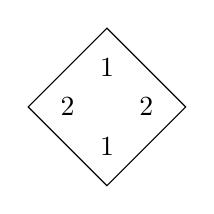
\begin{tikzpicture}[scale=1]
\draw (0.5,0) node              {$2$};
\draw (-0.5,0) node             {$2$};
\draw (0,0.5) node              {$1$};
\draw (0,-0.5) node             {$1$};
\draw (1,0) -- (0,1) -- (-1,0) -- (0, -1) -- cycle;
\end{tikzpicture}
    \caption{Hodge diamond of $\check{S}$}
    \label{S_check_diamond}
  \end{subfigure}
  \hfill
  \begin{subfigure}[b]{0.4\textwidth}
 \centering 
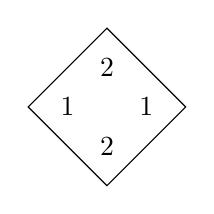
\begin{tikzpicture}[scale=1]

\draw (0.5,0) node              {$1$};
\draw (-0.5,0) node             {$1$};
\draw (0,0.5) node              {$2$};
\draw (0,-0.5) node             {$2$};
\draw (1,0) -- (0,1) -- (-1,0) -- (0, -1) -- cycle;
\end{tikzpicture}

    \caption{Hodge diamond of ${(S,\calF_S)}$}
    \label{S_diamond}
  \end{subfigure}
  \caption{Mirror partners}
\end{figure}






\end{document}